\subsection{Code analysis}
To get a better understanding of how the malicious application was build a code analysis was performed using JadX.
The process and results of the code analysis are described in this chapter.

On first glance it became obvious that the people behind the application obfuscated the code.
This meant that the code was difficult to understand.
Because of this it was possible to get an idea of what the code did, but it was not possible to say with certainty that it was correct.

In the code it was possible to confirm a lot of the permissions that were described in subchapter 4.1.2.1.
Within the obfuscated code the following aspects of the application might have been traced:

\texttt{The application can read files.}
\newline \texttt{The application can read your contacts.}
\newline \texttt{The application can record your calls.}
\newline \texttt{The application can find your location.}
\newline \texttt{The application can record audio.}
\newline \texttt{The application can record video.}
\newline \texttt{The application can execute shell commands.}
\newline \texttt{The application can read SMS messages.}
\newline \texttt{The application can send SMS messages.}
\newline \texttt{The application can start up when the phone boots.}
\newline \texttt{The application can send information.}

In the code the word “keylogger” was present.
This makes it very likely that the application contains a keylogger.
The code for the keylogger has been described below:

\begin{figure}[H]
    \centering
    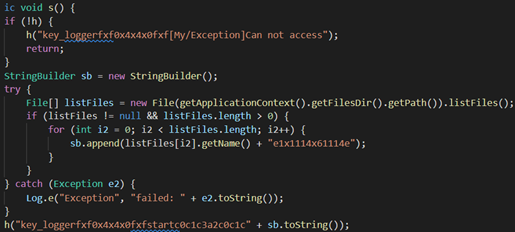
\includegraphics[width=1\textwidth]{CodeAnalysis2.png}
    \caption{Potential keylogger in the code}
    \label{jordy-keylogger}
\end{figure}

In the code there is a mention of an internet socket address.
The code described below shows there is a high likelihood that the malicious application sends data through a network socket to the previously mentioned command and control server. 

\begin{figure}[H]
    \centering
    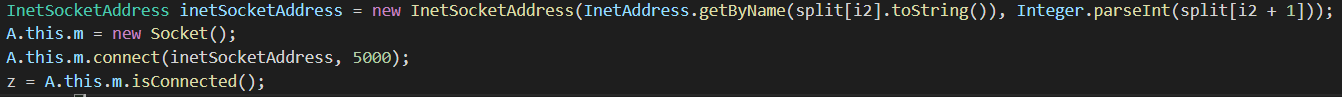
\includegraphics[width=1\textwidth]{CodeAnalysis.png}
    \caption{Potential network socket in the code}
    \label{jordy-networksocket}
\end{figure}